\documentclass[12pt]{article}
\usepackage[hmargin=3cm,vmargin=3.5cm]{geometry}

\usepackage[utf8]{inputenc}
\usepackage[french]{babel}
\usepackage[T1]{fontenc}
\usepackage{lmodern}

% Intégration de code Matlab
\usepackage[framed, numbered]{matlab-prettifier}

\usepackage{xcolor}
\usepackage{graphicx}
\usepackage{float}
\usepackage{amsmath}

\usepackage[justification=centering]{caption}

\graphicspath{ {F:/Travail/2A SRI\Commande de Robot/TP commande de robot} }

\title{Compte rendu de TP\\ \textbf{Commande articulaire d'un robot manipulateur de type RP}}
\author{Fleytoux Yoann , Aurélien Bernier Levalois}
\date{21 novembre 2016}


% Document
\begin{document}
\maketitle


% Table des matières
\tableofcontents
\vspace{0.6cm}


\section{Travail demandé}
 
\subsection{Prise en main de l'outil de simulation et calculs préliminaires}
\smallbreak
\medbreak
\textbf{1.}Relever l'évolution temporelle des profils de consigne

\smallbreak
Simulink
\begin{flushleft}
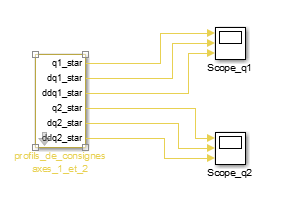
\includegraphics[width=\textwidth,height=\textheight,keepaspectratio]{1_1.PNG}
\end{flushleft}

$Scope_q1$: on peut observer le profil de position, vitesse et accélération de q1
\begin{flushleft}
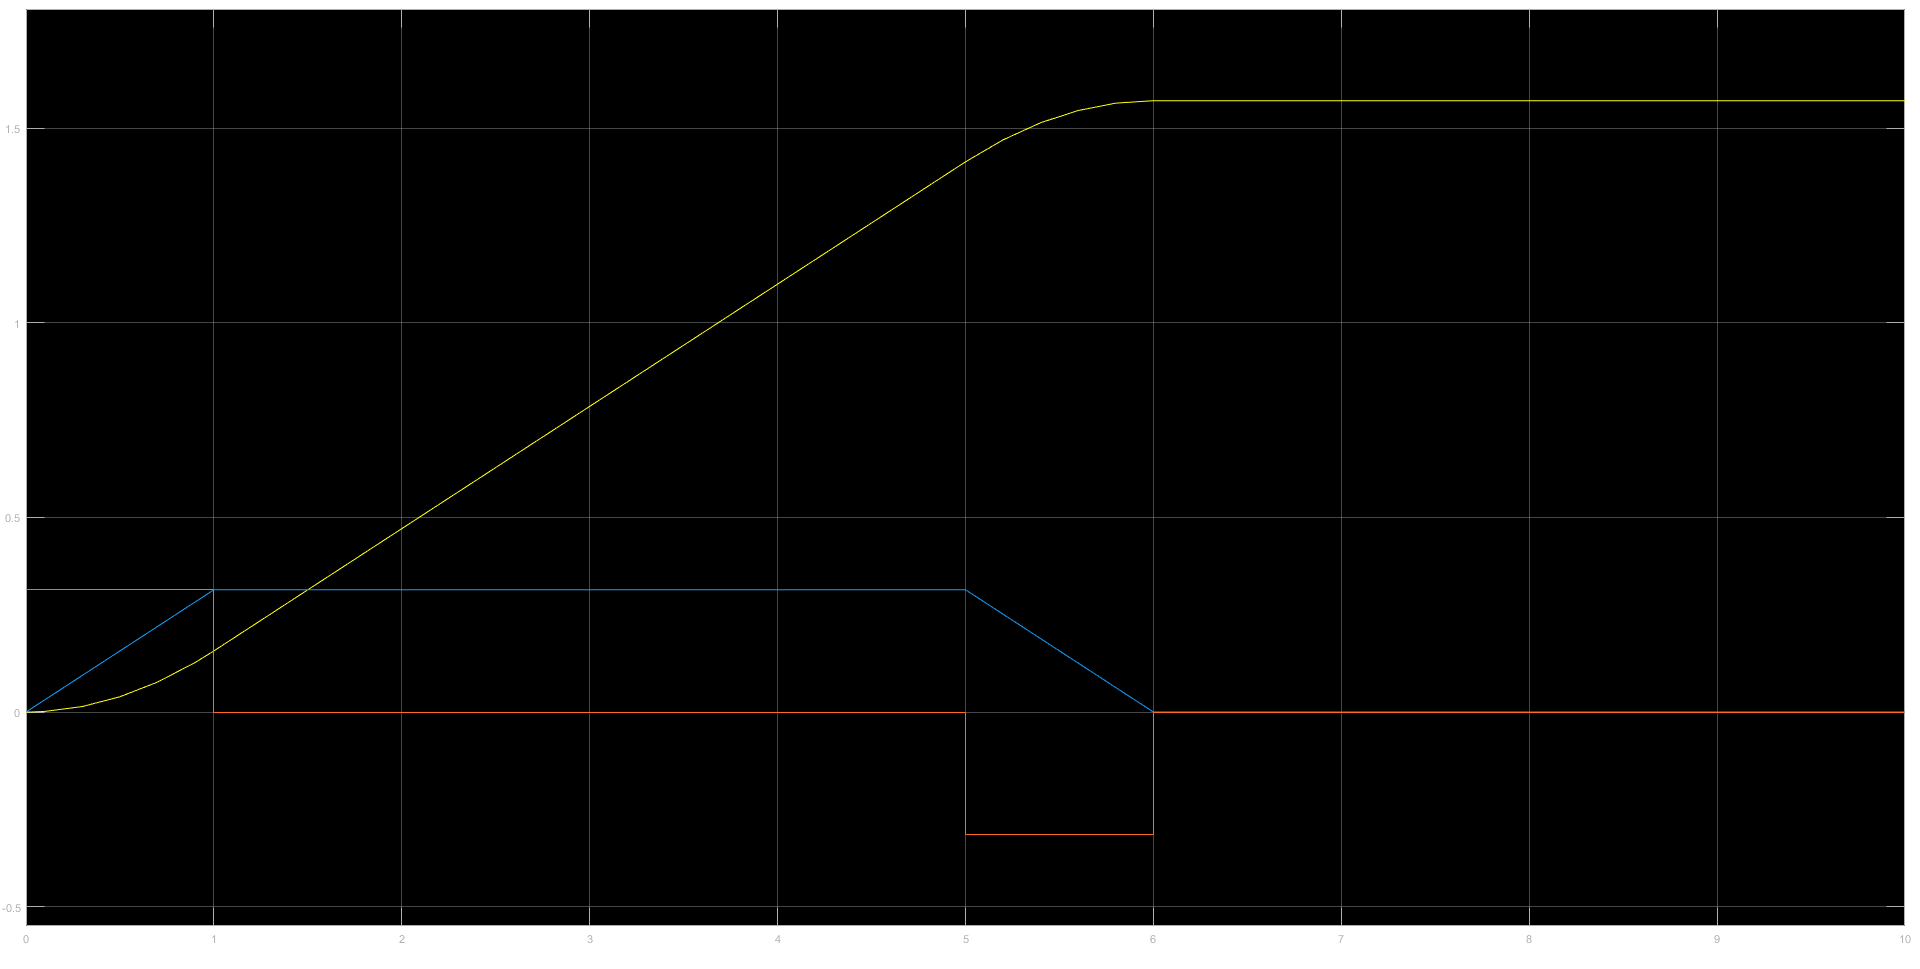
\includegraphics[width=\textwidth,height=\textheight,keepaspectratio]{1_1_q1.PNG}
\end{flushleft}

\clearpage
$Scope_q2$: on peut observer le profil de position, vitesse et accélération de q2
\begin{flushleft}
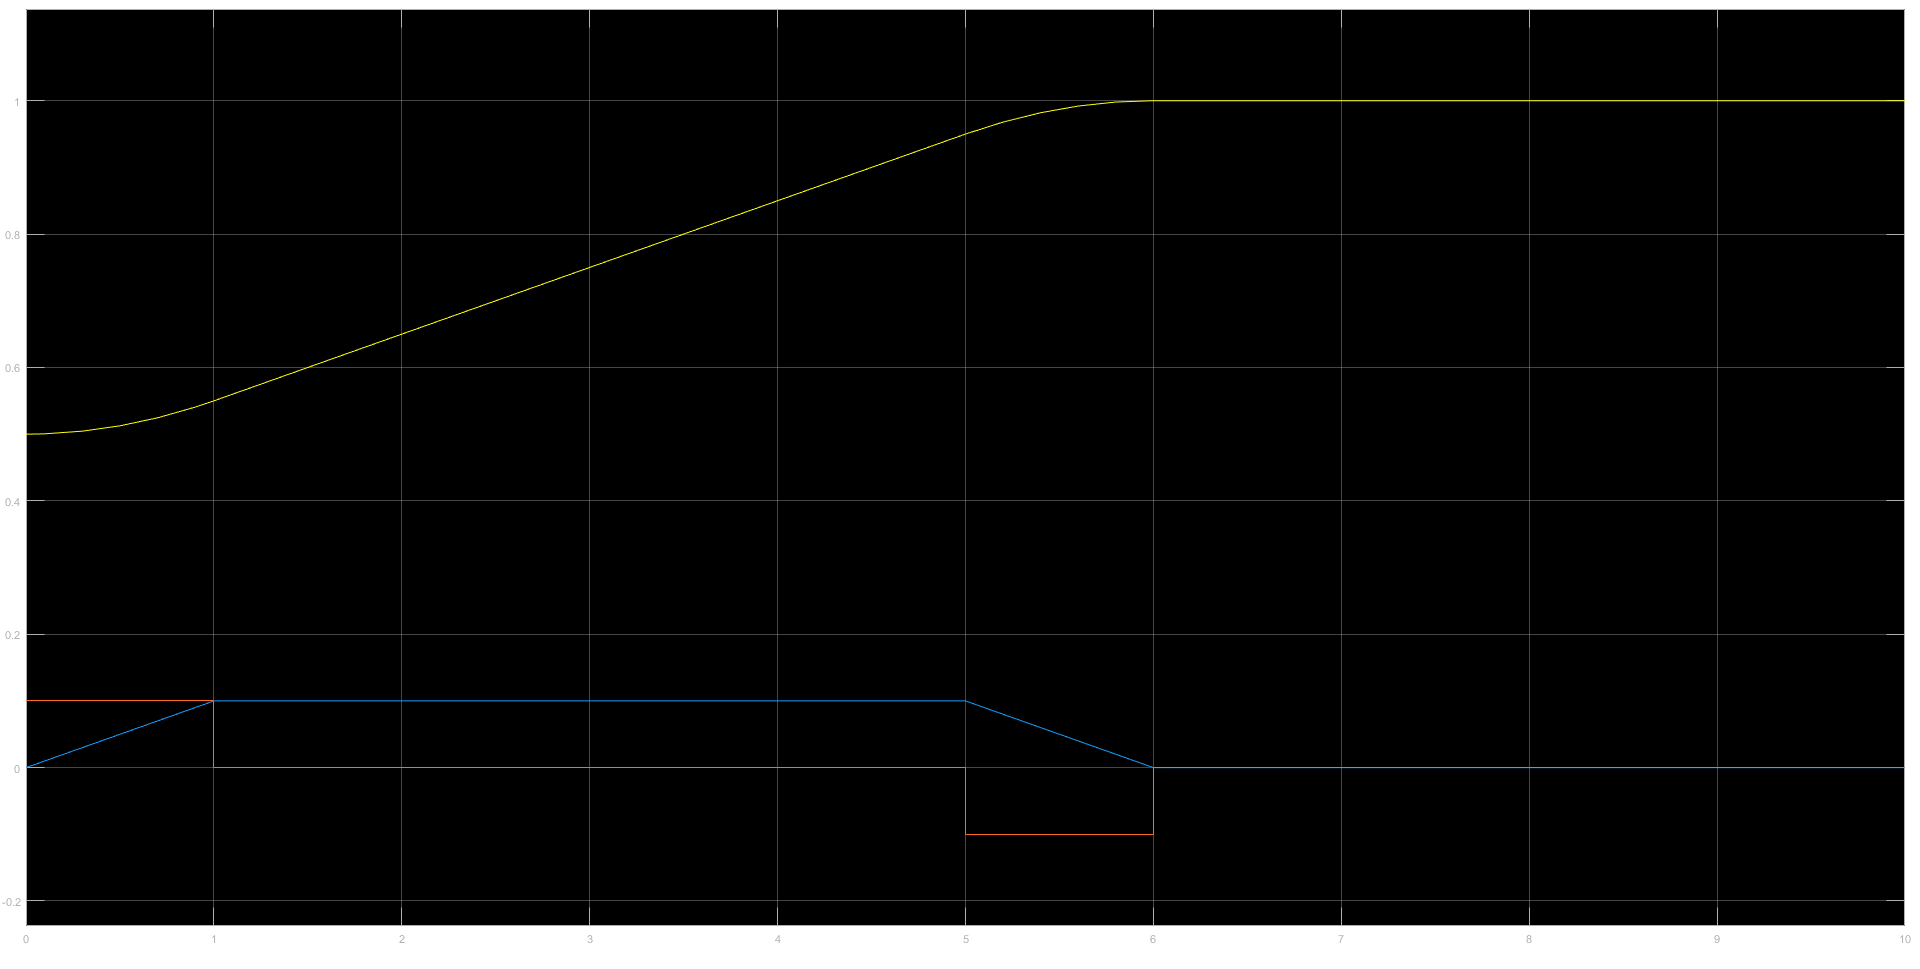
\includegraphics[width=\textwidth,height=\textheight,keepaspectratio]{1_1_q2.PNG}
\end{flushleft}

\textbf{2.}
\begin{lstlisting}[style=Matlab-editor]

m=15

Km_R = 0.3;

Beff = 1/80;

Jm = 1/100;

R = [1/200 1/30 1];

Jeff200 = Jm+(R(1)^2)*m;
Jeff30 = Jm+R(2)^2*m;
Jeff1 = Jm+R(3)^2*m;

\end{lstlisting}

\subsection{Commande en vitesse de type PD}
\textbf{3.} On cherche les coefficients K et KD de la loi de commande Proportionnelle Dérivée, pour $di(t)=0$, confère à la boucle fermée un amortissement unité $\zeta=1$ et une erreur de vitesse $/epsilon_1i$ donnée en réponse à une consigne rampe 
$\theta_{mi}^{*}(t)=\theta_{mi}^{1}t*U(t)\\$

avec $
wn=4 \\
K =(wn^2)*Jeff/(Km/R)=16*Jeff/(Km/R)\\
KD =((K/2)-(Beff/(Km/R)))=(8*Jeff-Beff)/(Km/r)
$

\textbf{4.}\\
a)
\begin{lstlisting}[style=Matlab-editor]
Ti = 0.8
zeta=1
wn=4

K200 =(wn^2)*Jeff200/Km_R
K30 =(wn^2)*Jeff30/Km_R
K1 =(wn^2)*Jeff1/Km_R

KD200 = ((K200/2)-(Beff/Km_R))
KD30 = ((K30/2)-(Beff/Km_R))
KD1 = ((K1/2)-(Beff/Km_R))
\end{lstlisting}
Avec r=1/200 Jeff= 1/100+15/40000=0.010375; on trouve K=0.5533 et KD=0.2350\\
Avec r=1/30  Jeff= 2/75=0.02666666666; on trouve K=1.4222 et KD=0.6694\\
Avec r=1     Jeff= 1/100+15=15.01; on trouve K=800.5333 et KD=400.2250\\

b) lieux de transfert de la boucle ouverte avant correction:
\begin{lstlisting}[style=Matlab-editor]
G_200=tf(1,[Jeff200 Beff 0])
G_30=tf(1,[Jeff30 Beff 0])
G_1=tf(1,[Jeff1 Beff 0])

(on suppose que d=1)

BO_200=series((Km_R-R(1)),G_200)
BF_200=feedback(K200*BO_200,tf([KD200 0],1))

BO_30=series((Km_R-R(2)),G_30)
BF_30=feedback(K30*BO_30,tf([KD30 0],1))

BO_1=series((Km_R-R(3)),G_1)
BF_1=feedback(K1*BO_1,tf([KD1 0],1))

margin(BO_200);
title('Marge de phase et marge de gain');
hold on;
margin(BF_200);
legend('BO_200','BF_200');
hold off;

figure
margin(BO_30);
title('Marge de phase et marge de gain');
hold on;
margin(BF_30);
legend('BO_30','BF_30');

figure
margin(BO_1);
title('Marge de phase et marge de gain');
hold on;
margin(BF_1);
legend('BO_1','BF_1');

\end{lstlisting}

\clearpage
$r=1/200$
\begin{flushleft}
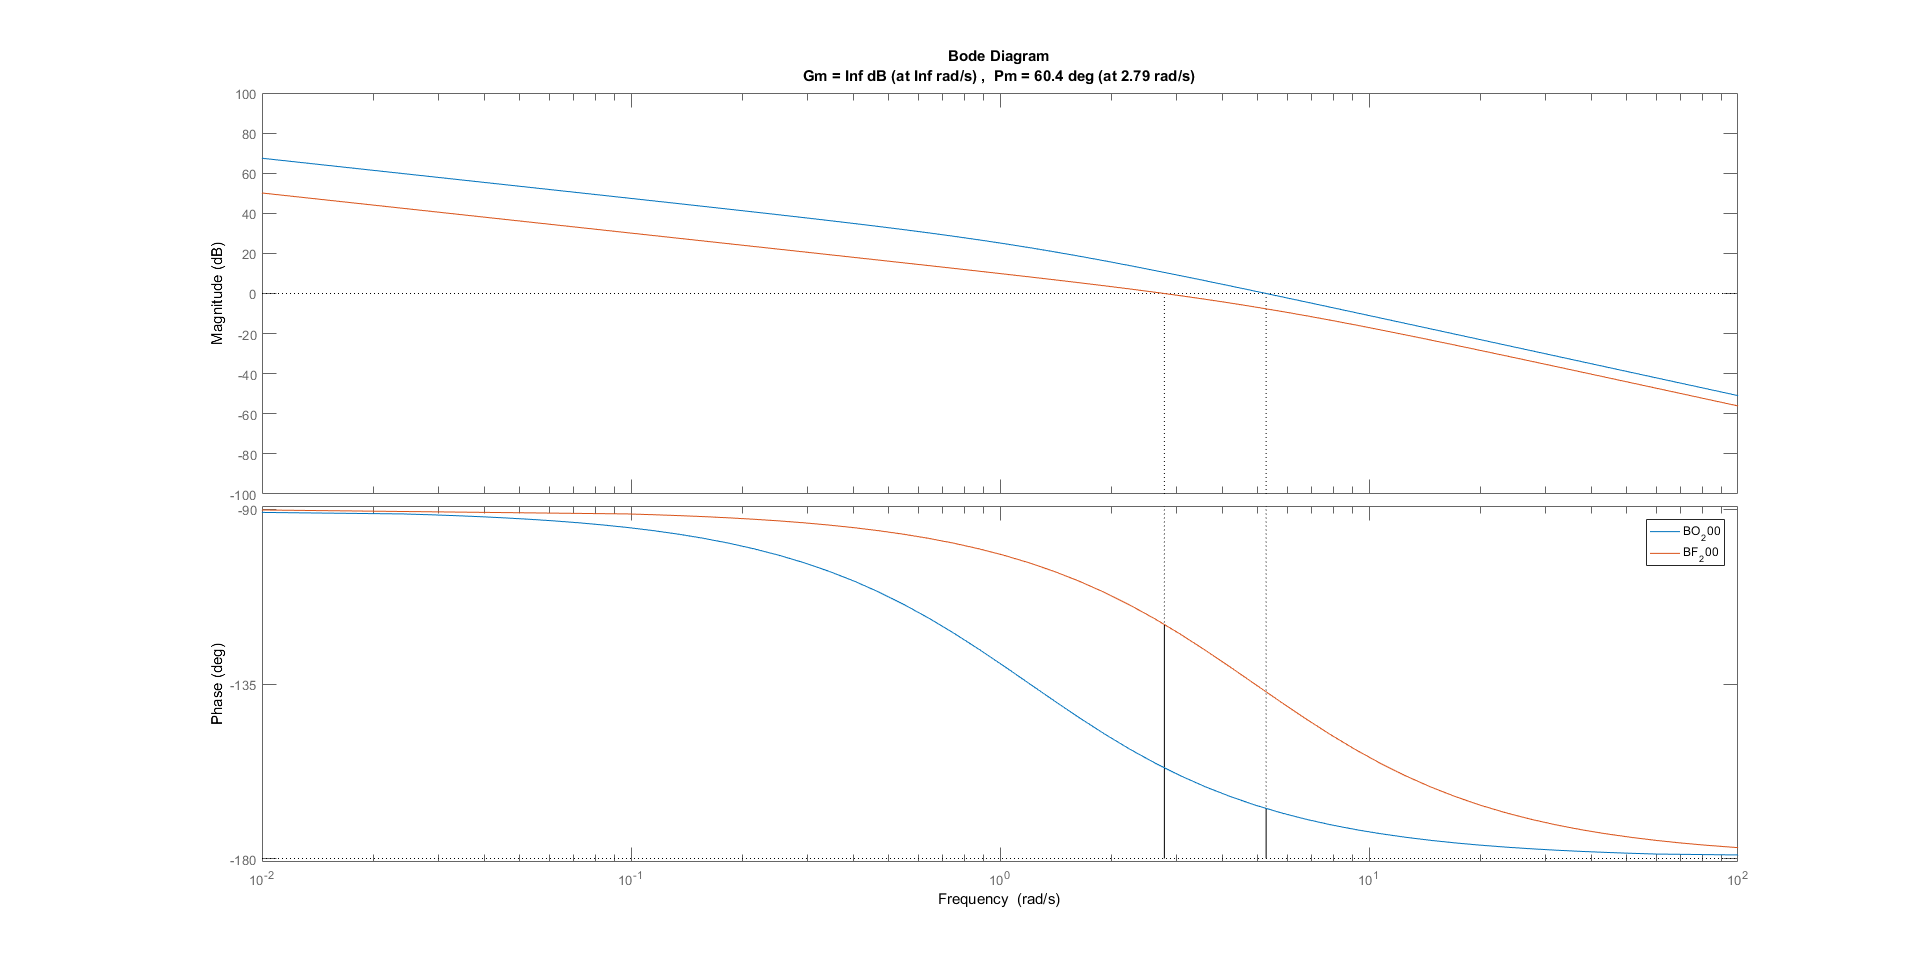
\includegraphics[width=\textwidth,height=\textheight,keepaspectratio]{Bode_200.PNG}
\end{flushleft}

$r=1/30$:
\begin{flushleft}
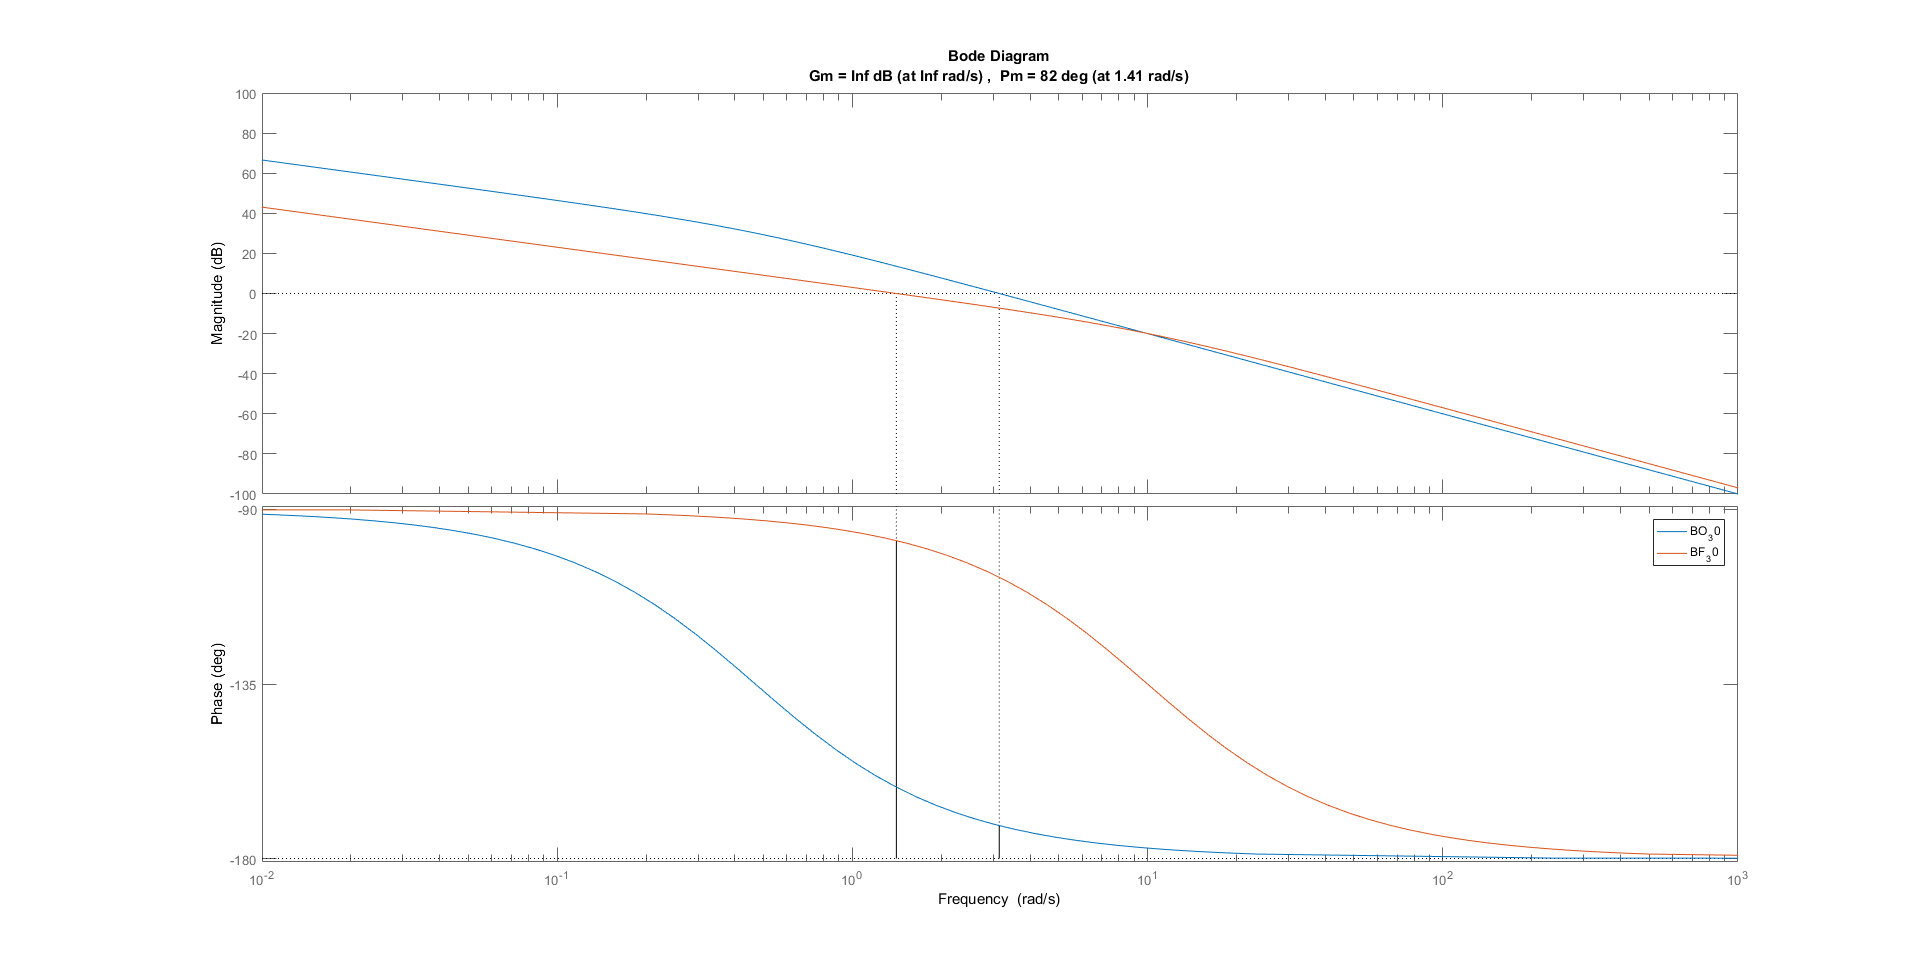
\includegraphics[width=\textwidth,height=\textheight,keepaspectratio]{Bode_30.PNG}
\end{flushleft}

\clearpage
$r=1/200$
$r=1$: 
\begin{flushleft}
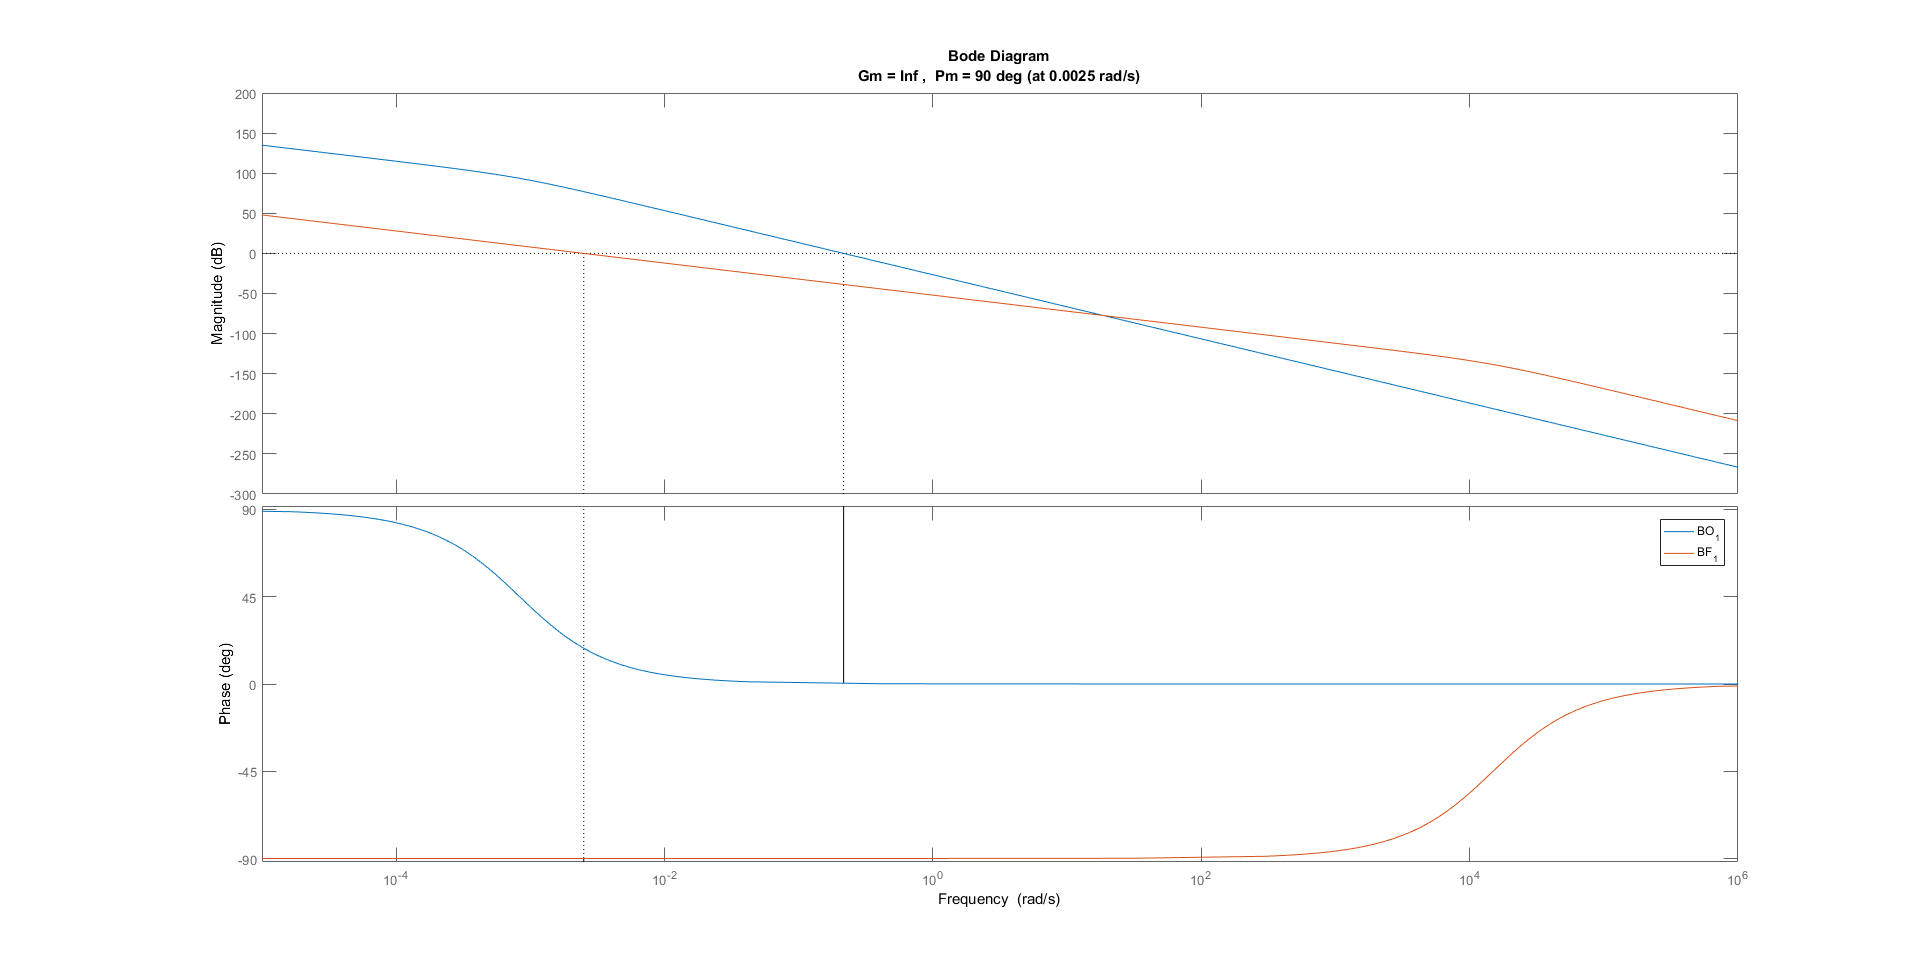
\includegraphics[width=\textwidth,height=\textheight,keepaspectratio]{Bode_1.PNG}
\end{flushleft}


\end{document}
